% !TeX TS-program = xelatex

\documentclass[compress, 8pt]{beamer}

\usepackage{presentationtemplate}
\usepackage[askip=3mm, bskip=3mm]{terminal}
\usepackage[linenosfontsize=\tiny, askip=3mm, bskip=3mm]{mylisting}
\usepackage{tikz}
\usetikzlibrary{positioning}
\usepackage{array}
\usepackage[table]{xcolor}

\renewcommand{\arraystretch}{1.2}

\title{Переменные}

\begin{document}

\frame[plain]{\titlepage}

\begin{frame}[fragile]

    \frametitle{Объявление переменной}

    Объявление переменной состоит из \textbf{типа} и \textbf{идентификатора} (имени).

    \begin{center}

        \verb|<type> <identifier>;|

        \begin{myinplacelisting}[minted language=cpp]
int a;
std::string s;
MyCustomType var;
        \end{myinplacelisting}

    \end{center}

    \begin{itemize}

        \item Первым символом идентификатора могут быть \verb|a-Z| или \verb|_|.

        \item Остальные символы идентификатора могут быть \verb|a-Z|,
            \verb|0-9| или \verb|_|.

        \item Идентификатор не должен совпадать с ключевым словом языка,
            например, \verb|int| или \verb|for|
            \footnote{Полный список ключевых слов языка C++:
                \url{https://en.cppreference.com/w/cpp/keyword}}.

        \item Идентификаторы регистрозависимы: \verb|var| и \verb|Var| ---
            различные имена перменнных.

    \end{itemize}

\end{frame}

\begin{frame}[fragile]

    \frametitle{Инициализация переменной}

    \textbf{Инициализация} переменной определяет, каким будет ее значение
    (т.е., чем будет заполнен соответствующий переменной участок памяти)
    после ее создания.

    Существует несколько видов инициализации:

    \begin{itemize}

        \item Copy-initialization: \\ \verb|= expression|
            \begin{myinplacelisting}[minted language=cpp]
bool b = false;
            \end{myinplacelisting}

        \item List-initialization: \\
            \verb|{}|, \verb|= {}|, \verb|= { initializer-list }| и др.
            \begin{myinplacelisting}[minted language=cpp]
int i {};
short s = { 1 };
            \end{myinplacelisting}

        \item Direct-initialization: \\ \verb|( expression )|
            \begin{myinplacelisting}[minted language=cpp]
float f(3.14);
            \end{myinplacelisting}

    \end{itemize}

\end{frame}

\begin{frame}[fragile]

    \frametitle{Инициализация переменной}

    Неконстантная переменная может быть не инициализирована.
    До C++26 чтение (т.е., любое использование) неинициализированной переменной
    считалось \textit{неопределенным поведением}, а начиная с C++26 ---
    \textit{ошибочным}
    \footnote{\url{https://github.com/Nekrolm/ubbook/blob/master/runtime/uninitialized.md}}.

    \hfill \break
    Константрая переменная должна быть инициализирована всегда.

\end{frame}

\begin{frame}[fragile]

    \frametitle{Инициализация переменной}

    \myinputlisting[minted language=cpp]
        {Presentations/4-Variables/}
        {uninit.cpp}

    \begin{terminalwindow}
        !\shellcommand{g++ \colorbox{yellow}{-Wall} uninit.cpp}!
uninit.cpp: In function ‘int !\textcolor{teal}{main}!()’:
unint.cpp:5:18: !\textcolor{orange}{warning:}! ‘i’ is used uninitialized [!\textcolor{orange}{-Wuninitialized}!]
    5 |     std::cout << !\textcolor{orange}{i}! << std::endl;
      |                  !\textcolor{orange}{\^{}}!
uninit.cpp:4:9: !\textcolor{cyan}{note}!: ‘i’ was declared here
    4 |     int !\textcolor{cyan}{i}!;
      |         !\textcolor{cyan}{\^{}}!
    \end{terminalwindow}

\end{frame}

\begin{frame}[fragile]

    \frametitle{Инициализация переменной}

    \myinputlisting[minted language=cpp]
        {Presentations/4-Variables/}
        {uninit-const.cpp}

    \begin{terminalwindow}
!\shellcommand{g++ uninit-const.cpp}!
uninit-const.cpp: In function ‘int !\textcolor{teal}{main}!()’:
uninit-const.cpp:2:15: !\textcolor{red}{error:}! uninitialized ‘const i’ [!\textcolor{red}{-fpermissive}!]
    2 |     const int !\textcolor{red}{i}!;
      |               !\textcolor{red}{\^{}}!
    \end{terminalwindow}

\end{frame}

\begin{frame}[fragile]

    \frametitle{Присваивание}

    \textbf{Присваиванием} значения переменной называется изменение ее
        значения при помощи оператора присваивания
        \footnote{Полный список операторов присваивания:
            \url{https://en.cppreference.com/w/cpp/language/operator\_assignment}}.

    \begin{myinplacelisting}[minted language=cpp]
int i = 0;  // initialization, not assignment
i = 1;      // simple assignment
i += 2;     // addition assignment
i *= 3;     // multiplication assignment

const char c = 'c';
c = 'd';    // compilation error
    \end{myinplacelisting}

\end{frame}

\begin{frame}[fragile]

    \frametitle{Область видимости переменной}

    Каждому объявлению переменной ставится в соответствие
    \textbf{область видимости} (scope)
    \footnote{\url{https://en.cppreference.com/w/cpp/language/scope}}.
    Переменная может использоваться только в пределах своей области
    видимости.

    \hfill \break
    Примеры областей видимости:

    \begin{itemize}
        \item Global scope
        \item Block scope
        \item Function parameter scope
        \item Namespace scope
    \end{itemize}

    \hfill \break
    Не допускается создавать более одной переменной с одним и тем же
    идентификатором в одной области видимости.


\end{frame}

\begin{frame}[fragile]

    \frametitle{Область видимости переменной}

    Глобальная область видимости (global scope):

    \begin{myinplacelisting}[minted language=cpp]
double d {};

d; // ok

int main() {
    double copy = d; // ok
}
    \end{myinplacelisting}

\end{frame}

\begin{frame}[fragile]

    \frametitle{Область видимости переменной}

    Block scope:

    \begin{myinplacelisting}[minted language=cpp]
void foo() {
    int i = 0;
    i; // ok
}

int main() {
    i; // compilation error

    {
        bool b;
        b; // ok
    }
    b; // compilation error

    for (int j = 0; j < 10; ++j) {
        j; // ok
    }
    j; // compilation error
}
    \end{myinplacelisting}

\end{frame}

\begin{frame}[fragile]

    \frametitle{Область видимости переменной}

    \begin{columns}[T]

        \begin{column}{0.5\textwidth}

            Function parameter scope:

            \begin{myinplacelisting}[minted language=cpp]
void foo(int x) {
    x; // ok
}

x; // compilation error
            \end{myinplacelisting}

        \end{column}

        \begin{column}{0.5\textwidth}

            Namespace scope:

            \begin{myinplacelisting}[minted language=cpp]
namespace X {
    std::string s;
    void foo() {
        s; // ok
    }
}

s; // compilation error
X::s; // ok
            \end{myinplacelisting}

        \end{column}

    \end{columns}

\end{frame}

\begin{frame}[fragile]

    \frametitle{Область видимости переменной}

    Области видимости могут быть вложенными:

    \begin{columns}[T]

        \begin{column}{0.5\textwidth}

            \begin{myinplacelisting}[minted language=cpp]
{
    const bool b = true;
    {
        {
            long l = {};
        }
        float f {};
    }
}
            \end{myinplacelisting}

        \end{column}

        \begin{column}{0.5\textwidth}

            \begin{myinplacelisting}[minted language=cpp]
namespace X {
    int a {};
    namespace Y {
            int a {};
    }
}

X::a;
X::Y::a;
            \end{myinplacelisting}

        \end{column}

    \end{columns}

\end{frame}

\begin{frame}[fragile]

    \frametitle{Область видимости переменной}

    \myinputlisting[minted language=cpp]
        {Presentations/4-Variables/}
        {same-identifier.cpp}

    \begin{terminalwindow}
!\shellcommand{g++ same-identifier.cpp}!
same-identifier.cpp: In function ‘int !\textcolor{teal}{main}!()’:
same-identifier.cpp:4:15: !\textcolor{red}{error}!: conflicting declaration ‘float a’
    4 |         float !\textcolor{red}{a}! {};
      |               !\textcolor{red}{\^{}}!
same-identifier.cpp:3:13: !\textcolor{cyan}{note}!: previous declaration as ‘int a’
    3 |         int !\textcolor{cyan}{a}! {};
      |             !\textcolor{cyan}{\^{}}!
    \end{terminalwindow}

\end{frame}

\begin{frame}[fragile]

    \frametitle{Storage duration}

    У каждой переменной есть свойство времени выполнения, которое называется
    \textbf{временем жизни}
    \footnote{\url{https://en.cppreference.com/w/cpp/language/lifetime}} (lifetime).
    Время жизни определяется моментом создания и уничтожения переменной.

    \hfill \break
    Минимальное время жизни контролируется свойством времени компиляции,
    которое называется \textbf{storage duration}
    \footnote{\url{https://en.cppreference.com/w/cpp/language/storage\_duration}}.
    Существуют следующие storage duration:

    \begin{itemize}
        \item static
        \item thread
        \item automatic
        \item dynamic
    \end{itemize}

\end{frame}

\begin{frame}[fragile]

    \frametitle{Storage duration}

    Automatic storage duration:

    \begin{myinplacelisting}[minted language=cpp]
{
    char c0 = {}; // <- c0's lifetime begins
    {
        char c1 = {}; // <- c1's lifetime begins
    } // <- c1's lifetime ends
} // <- c0's lifetime ends
    \end{myinplacelisting}

    Чаще всего автоматическое время хранения в памяти реализовано через
    структуру данных \textbf{LIFO stack}
    \footnote{\url{https://en.wikipedia.org/wiki/Stack-based\_memory\_allocation}}:

    \hfill \break

    \centering

    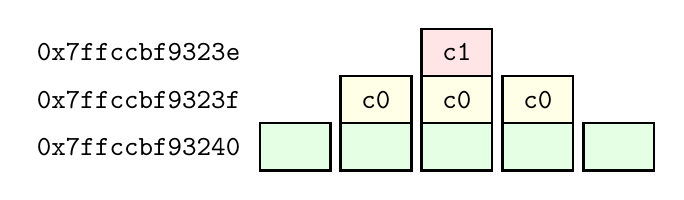
\begin{tikzpicture} [
        bytenode/.style={
            rectangle,
            thick,
            minimum width=9mm,
            minimum height=6mm
        }
    ]

        \node[bytenode] (addr0)                                 {\verb|0x7ffccbf93240|};
        \node[bytenode] (addr1) [above=-\pgflinewidth of addr0] {\verb|0x7ffccbf9323f|};
        \node[bytenode] (addr2) [above=-\pgflinewidth of addr1] {\verb|0x7ffccbf9323e|};

        \node[bytenode, draw, fill=green!10]    (bn00) [right=1mm of addr0]             {};
        \node[bytenode, draw, fill=green!10]    (bn01) [right=1mm of bn00]              {};
        \node[bytenode, draw, fill=yellow!10]   (bn11) [above=-\pgflinewidth of bn01]   {\verb|c0|};
        \node[bytenode, draw, fill=green!10]    (bn02) [right=1mm of bn01]              {};
        \node[bytenode, draw, fill=yellow!10]   (bn12) [above=-\pgflinewidth of bn02]   {\verb|c0|};
        \node[bytenode, draw, fill=red!10]      (bn22) [above=-\pgflinewidth of bn12]   {\verb|c1|};
        \node[bytenode, draw, fill=green!10]    (bn03) [right=1mm of bn02]              {};
        \node[bytenode, draw, fill=yellow!10]   (bn13) [above=-\pgflinewidth of bn03]   {\verb|c0|};
        \node[bytenode, draw, fill=green!10]    (bn04) [right=1mm of bn03]              {};

    \end{tikzpicture}

\end{frame}

\begin{frame}[fragile]

    \frametitle{Storage duration}

    Dynamic storage duration:

    \begin{myinplacelisting}[minted language=cpp]
int* i = new int(0);        // <- i's lifetime begins
float* f = new float(0.0);  // <- f's lifetime begins
delete i;                   // <- i's lifetime ands
delete f;                   // <- f's lifetime ends
    \end{myinplacelisting}

    Область оперативной памяти программы, в которой хранятся объекты
    с динамическим временем хранения, называется \textbf{кучей}
    \footnote{\url{https://en.wikipedia.org/wiki/Memory\_management\#Manual\_memory\_management}}
    (heap).

    \hfill \break
    \centering

    \begin{tabular}{|m{2cm}|m{10mm}|m{1cm}|m{5mm}|m{1.5cm}|}
        \hline
        \hfill &
        \cellcolor{red!10} \verb|f| &
        \hfill &
        \cellcolor{green!10} \verb|i| &
        \hfill \\
        \hline
    \end{tabular}
    \begin{tabular}{m{2cm}m{10mm}m{1cm}m{5mm}m{1.5cm}}
        \hfill &
        \texttt 0x7ffe0c2c1a90 &
        \hfill &
        \texttt 0x7ffe0c2c1167 &
        \hfill \\
    \end{tabular}

\end{frame}

\begin{frame}[fragile]

    \frametitle{Storage duration}

    Static storage duration:

    \begin{myinplacelisting}[minted language=cpp]
int i {};

namespace X {
    char c {};
}

void foo() {
    static float f {};
}
    \end{myinplacelisting}

    Время жизни переменных со статическим временем хранения
    совпадает с временем выполнения программы.

\end{frame}

\begin{frame}[fragile]

    \frametitle{Linkage}

    \textbf{Связывание}
    \footnote{\url{https://en.cppreference.com/w/cpp/language/storage\_duration\#linkage}}
    (linkage) переменной определяет возможность ее использования из другой
    \textit{единицы трансляции} (другого *.cpp-файла).

    \hfill \break
    Различают следующие виды связывания:

    \begin{itemize}
        \item внутреннее (internal linkage)
        \item внешнее (external linkage)
    \end{itemize}

\end{frame}

\begin{frame}[fragile]

    \frametitle{Linkage}

    External linkage:

    \begin{columns}[T]
        \begin{column}{0.5\textwidth}

            \myinputlisting[minted language=cpp]
                {Presentations/4-Variables/extern/}
                {foo.h}

            \myinputlisting[minted language=cpp]
                {Presentations/4-Variables/extern/}
                {foo.cpp}

        \end{column}
        \begin{column}{0.5\textwidth}

            \myinputlisting[minted language=cpp]
                {Presentations/4-Variables/extern/}
                {main.cpp}

        \end{column}
    \end{columns}

    \begin{terminalwindow}
!\shellcommand{g++ main.cpp foo.cpp}!
!\shellcommand{./a.out}!
1
    \end{terminalwindow}

\end{frame}

\end{document}
